\documentclass[12pt, titlepage]{article}

\usepackage{tabularx}
\usepackage{booktabs}

\usepackage[final]{pdfpages}
\setboolean{@twoside}{false}

\input{../Comments}
\input{../Common}

\begin{document}

\title{GenderMag Report: \progname} 
\author{\authname}
\date{\today}
	
\maketitle

\pagenumbering{roman}

\section{Revision History}

\begin{tabularx}{\textwidth}{p{3cm}p{2cm}X}
\toprule {\bf Date} & {\bf Version} & {\bf Notes}\\
\midrule
2025-03-18 & 1.0 & Initial version.\\
\bottomrule
\end{tabularx}

~\newpage

\section{Symbols, Abbreviations and Acronyms}

\renewcommand{\arraystretch}{1.2}
\begin{table}[h!]
  \vspace{5pt}
  \begin{tabular}{l l} 
    \toprule		
    \textbf{Symbol} & \textbf{Description} \\
    \midrule 
    GM & GenderMag. \\
    PDF & Portable Document Format. \\
    UC & Use Case. \\
    UI & User Interface. \\
    \bottomrule
  \end{tabular}\\
\end{table}
\newpage

\tableofcontents

\newpage

\pagenumbering{arabic}
\newpage

\section{Introduction} %reference needed
This document details the results of the usage of the GenderMag method to evaluate gender
inclusivity as an aspect of ScoreGen's usability. It uses empirically based personas to simulate
the software system's use from diverse perspectives, revealing design issues that might be missed.\\
This document is organized into sections covering use cases, customized personas, reporting forms, 
and the design changes implemented based on the GenderMag evaluation. Each section provides a focused 
look at how GenderMag helps improve software inclusiveness.

\section{Methodology}
The team followed the prescribed GenderMag evaluation methodology, engaging collaboratively throughout the process. 
In each of the two sessions, we formed our own individual perspectives and insights and then consolidated them in 
unified decisions on whether a persona would or would not formulate/undertake a specific subgoal/action. This approach 
was chosen as it maximized the diversity of perspectives and minimized the risk of bias from any one team member.

\section{Use Cases}
The GenderMag method was applied to the following two use cases of the software system:
\begin{enumerate}
    \item[UC1.] Recording audio
    \item[UC2.] Generating sheet music from audio
\end{enumerate}

\section{Customized Personas}
\subsection{Abi}
Abi is designed to represent users with facet values often seen in females, such as comprehensive 
information processing and higher risk aversion. For more details, see the full persona:
\href{Personas/abi.pdf}{View the Abi Persona PDF}.

\subsection{Tim}
Tim represents users with facet values commonly found among males, characterized by a selective 
information processing style and an impulse for exploring new functionalities. For additional 
details, see the full persona:
\href{Personas/tim.pdf}{View the Tim Persona PDF}.

\section{Report Forms}
The GenderMag method uses three types of reporting forms: subgoal, action, and result. The subgoal reporting
form is used to document the steps that the persona formulates themselves and tries to achieve, while the action
reporting form is used to document the actions the persona takes to achieve the subgoals. The
subgoal reporting form is filled out first, followed by the action reporting form. After all subgoal and action 
reporting forms are filled, the results reporting form tallies the results and identifies general UI issues and/or 
gender-inclusion issues with the application.\\
All raw reporting forms for each use case are provided in this document.
\subsection{Use Case 1 Reports}
Use Case 1 is the recording audio use case. The Abi persona reflects
facet values commonly seen in women, such as high risk-aversion, low self-
efficacy, and so on.
\subsubsection{Subgoal Reporting Forms}
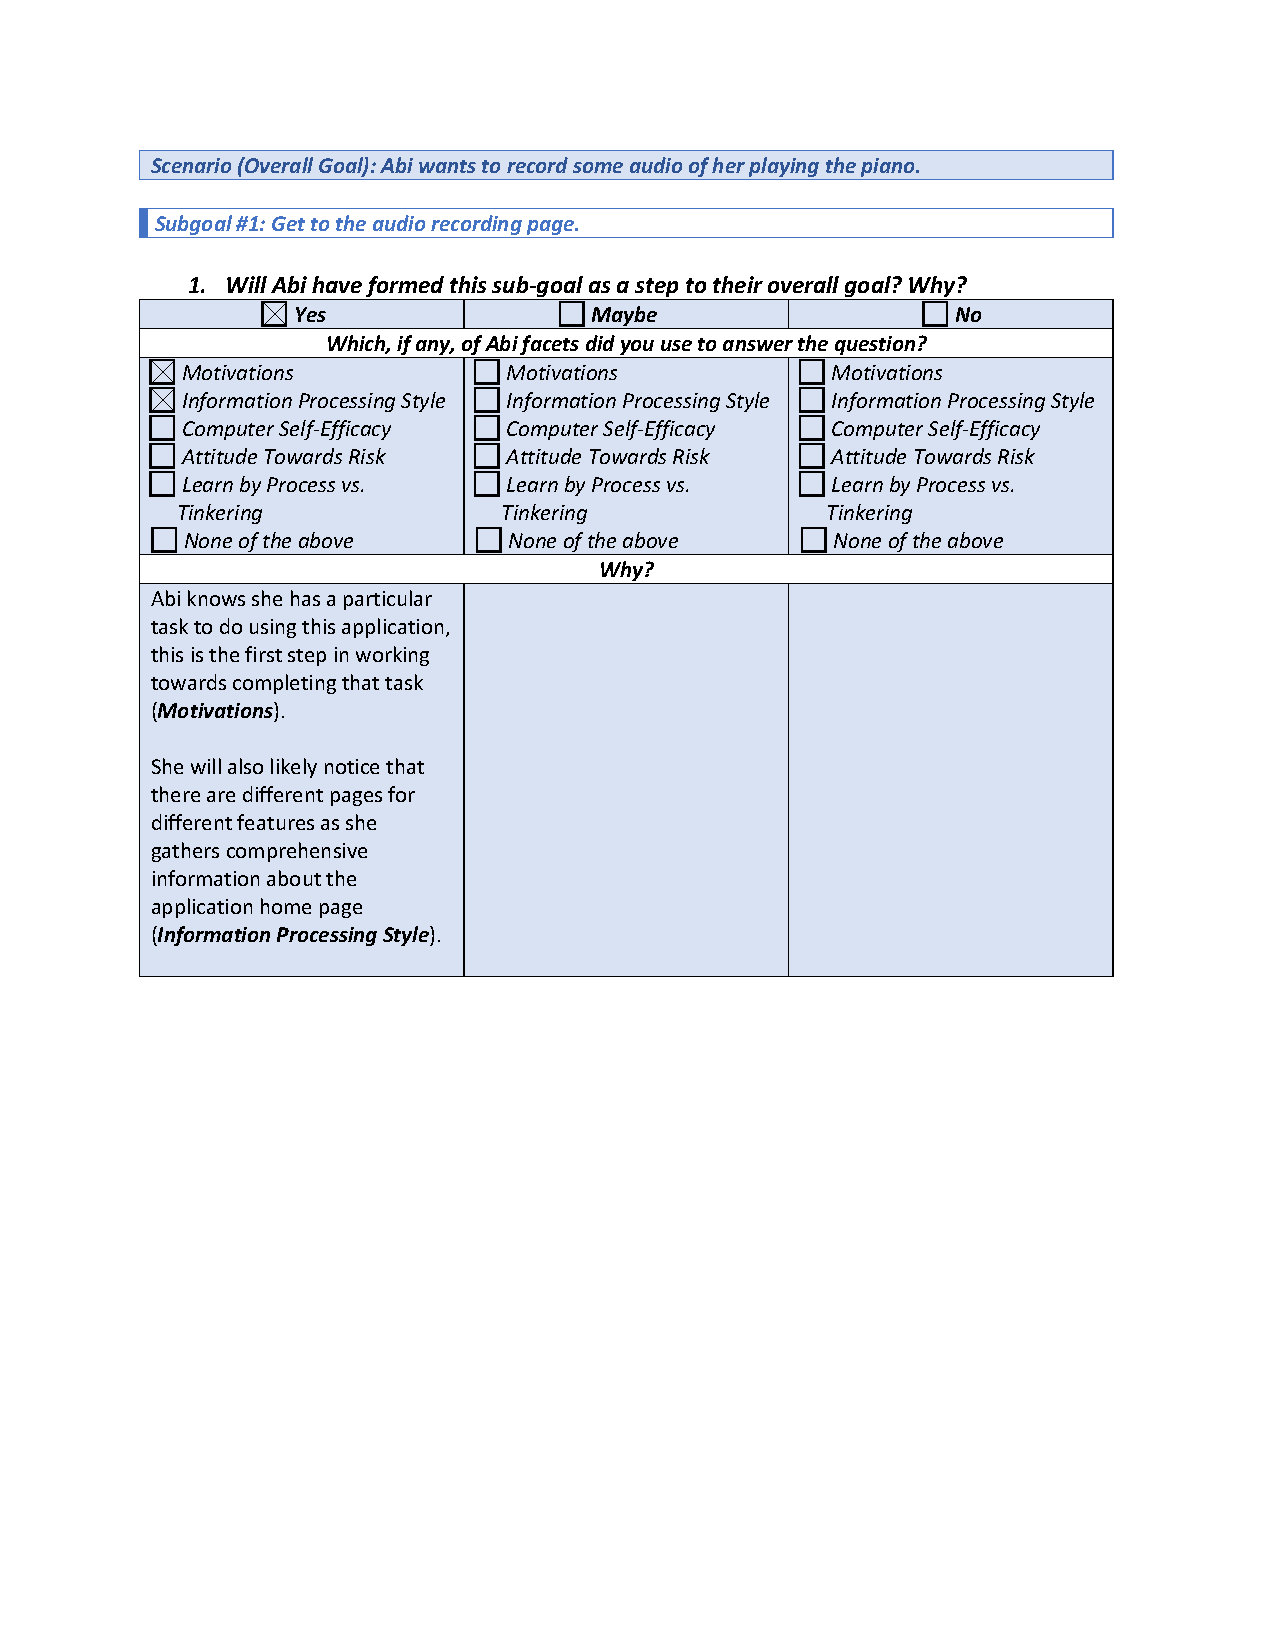
\includepdf[pages=-]{ReportForms/SubgoalForms/abi-subgoals.pdf}
\subsubsection{Action Reporting Forms}
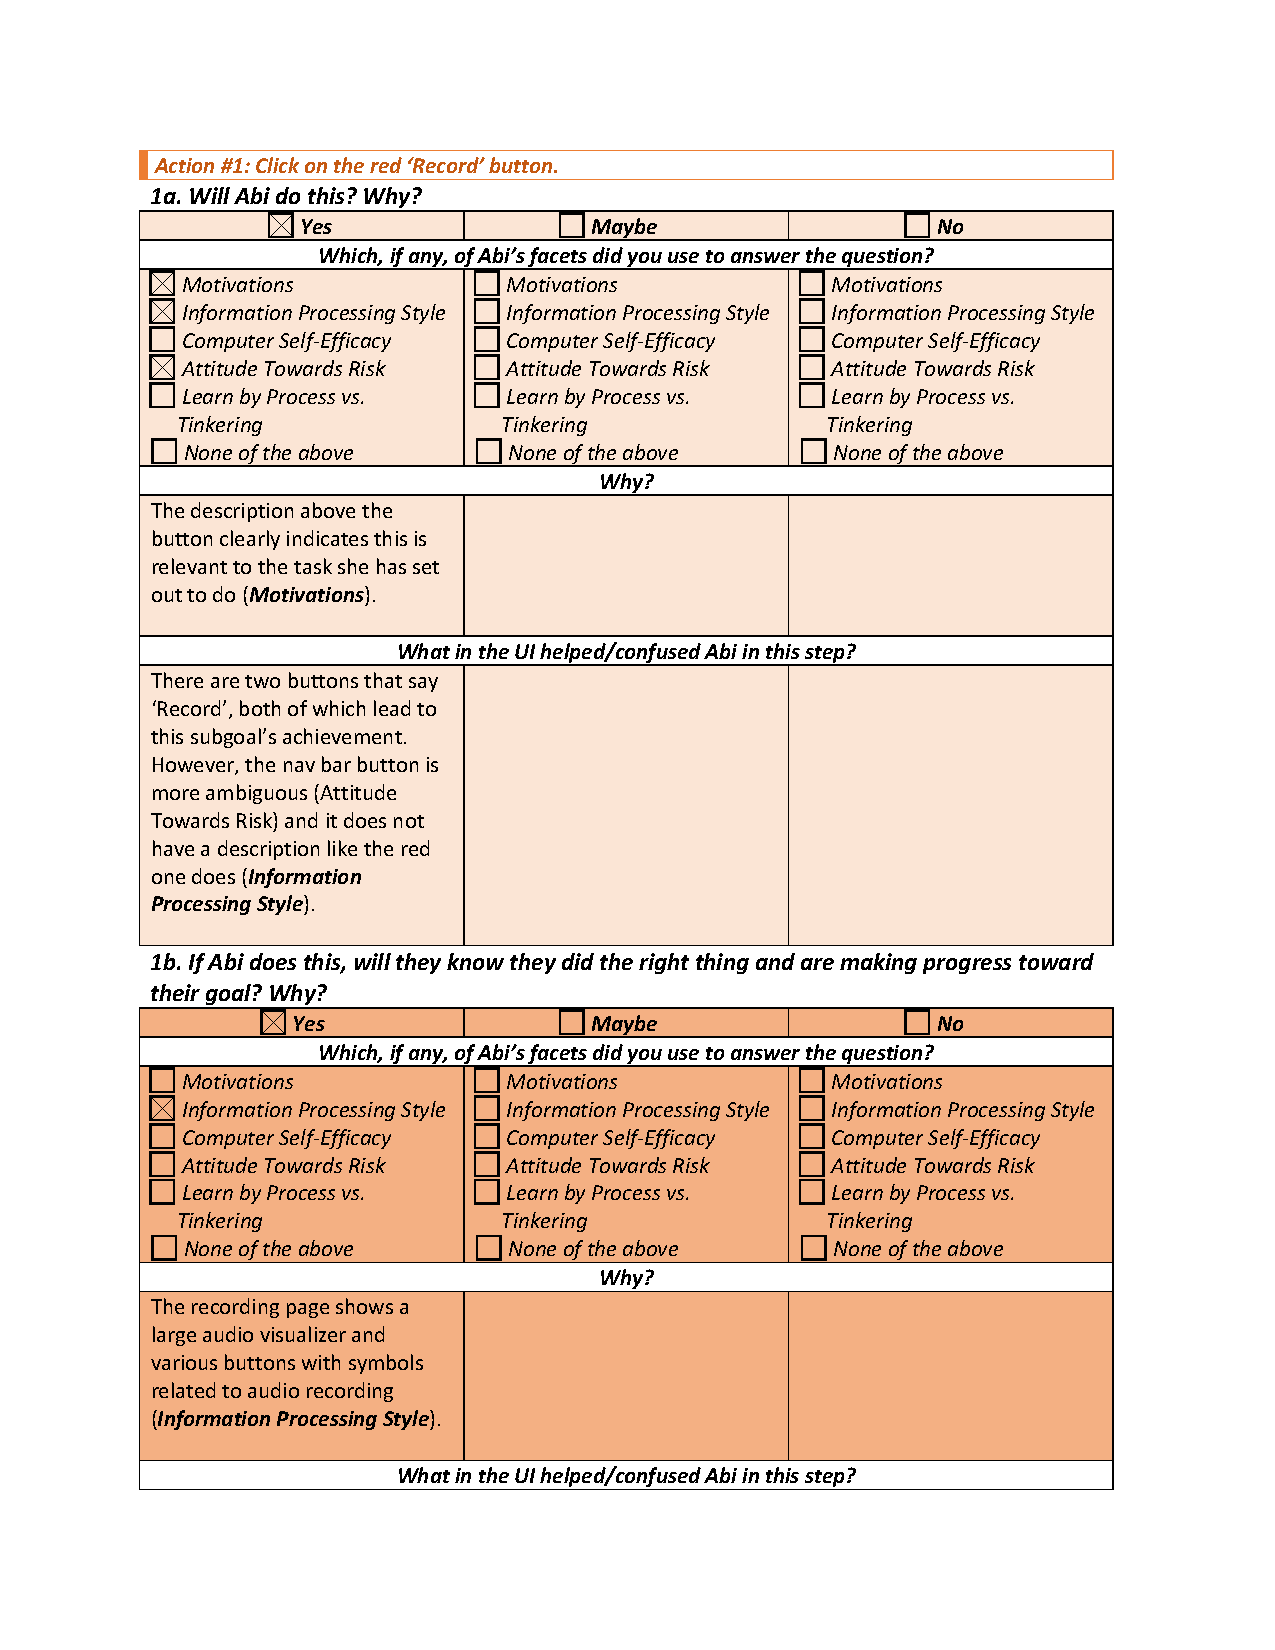
\includepdf[pages=-]{ReportForms/ActionForms/abi-actions.pdf}
\subsubsection{Results Reporting Form}
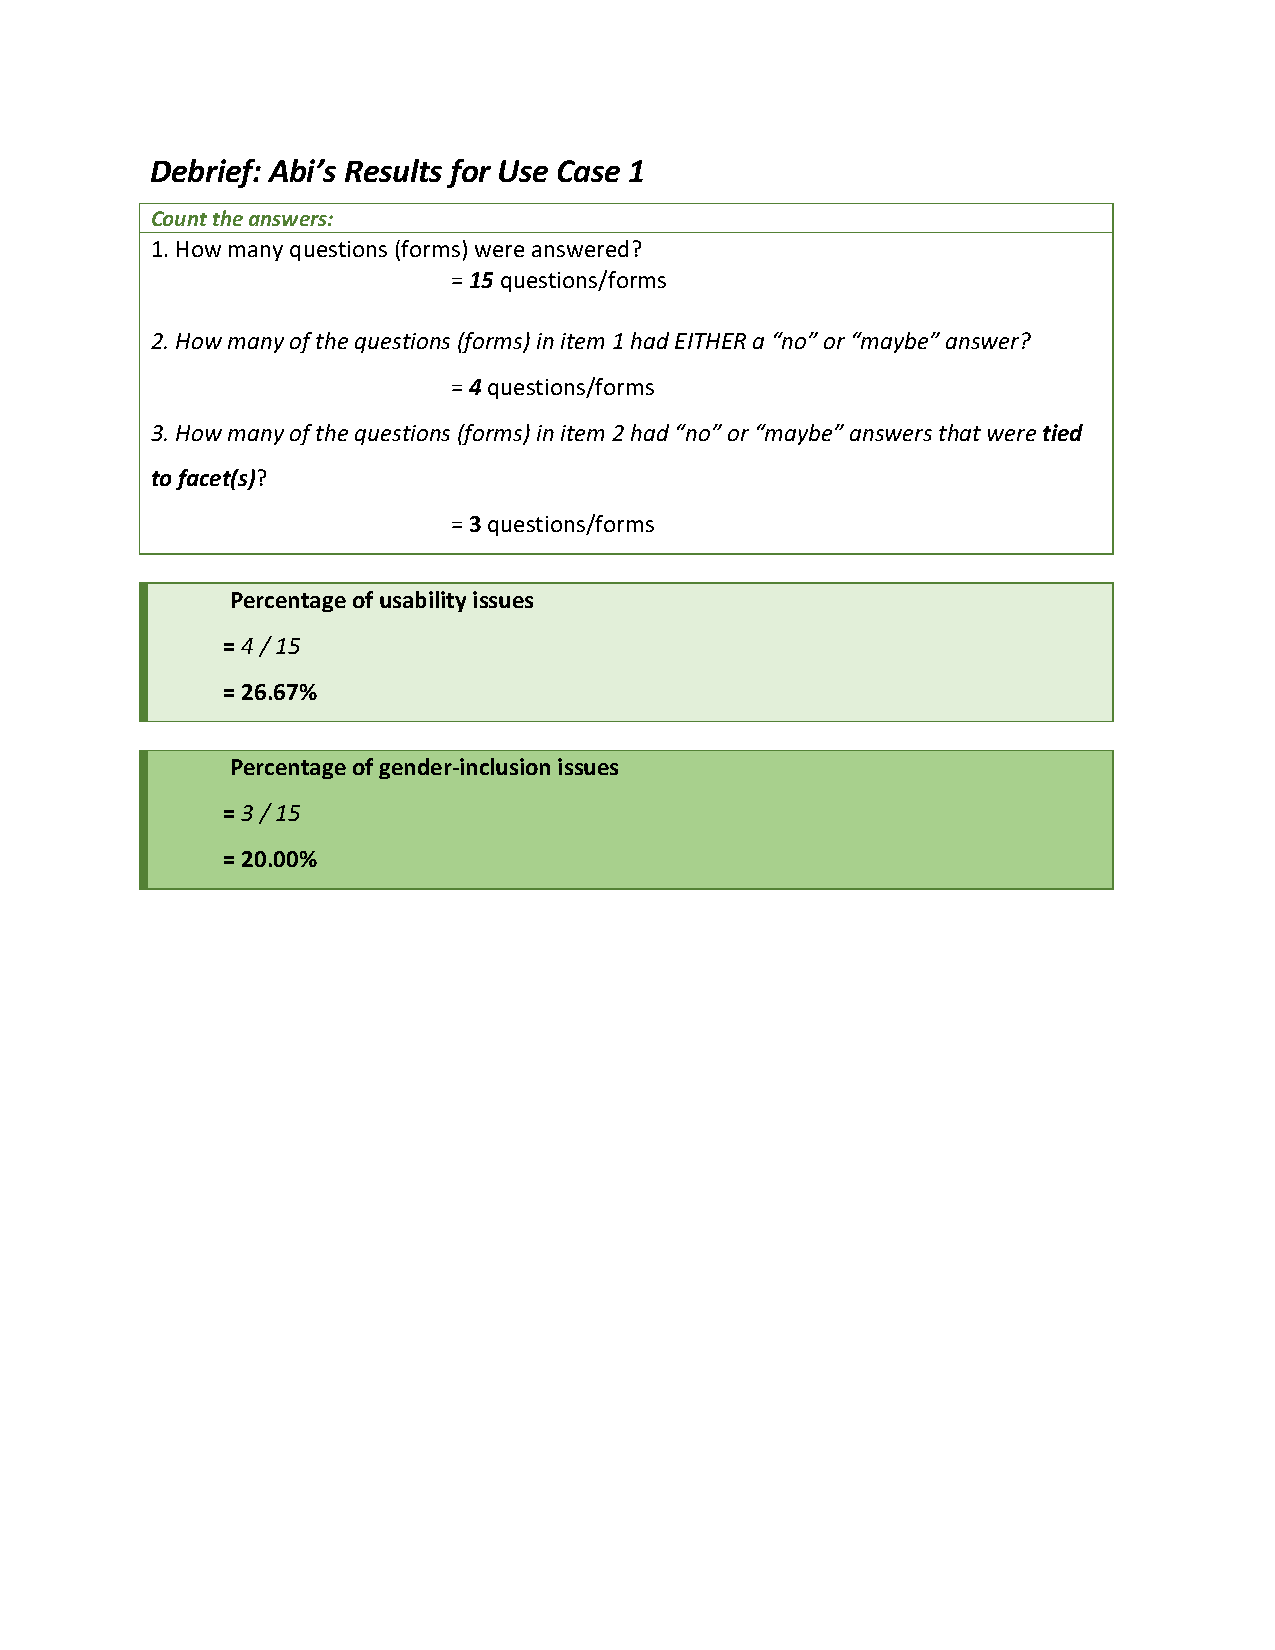
\includepdf[pages=-]{ReportForms/ResultsForms/abi-results.pdf}

\subsection{Use Case 2 Reports}
Use Case 2 is the generating sheet music from audio use case. The Tim persona reflects
facet values strongly associated with men. Significantly, Tim and Abi have very similar
backgrounds;
they are primarily different when it comes to the way they reflect the 5 facets.
\subsubsection{Subgoal Reporting Forms}
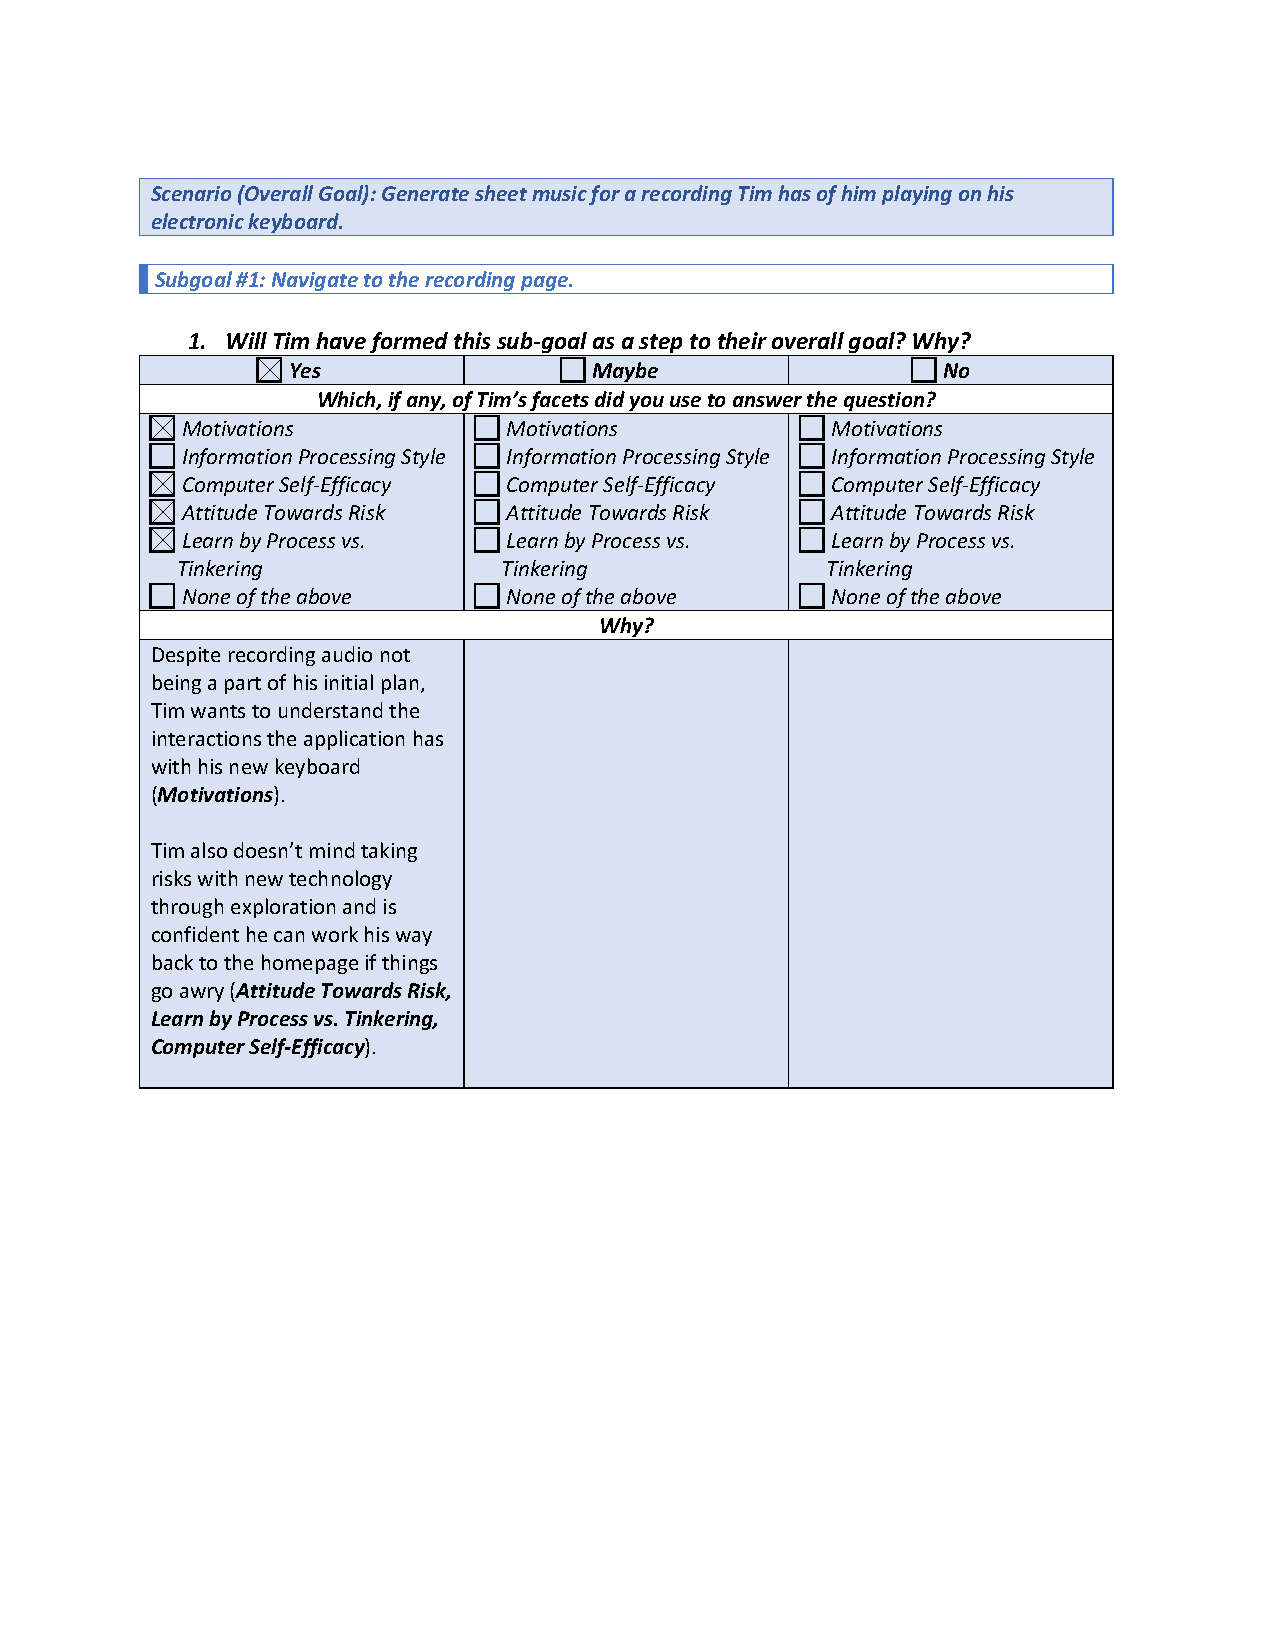
\includepdf[pages=-]{ReportForms/SubgoalForms/tim-subgoals.pdf}
\subsubsection{Action Reporting Forms}
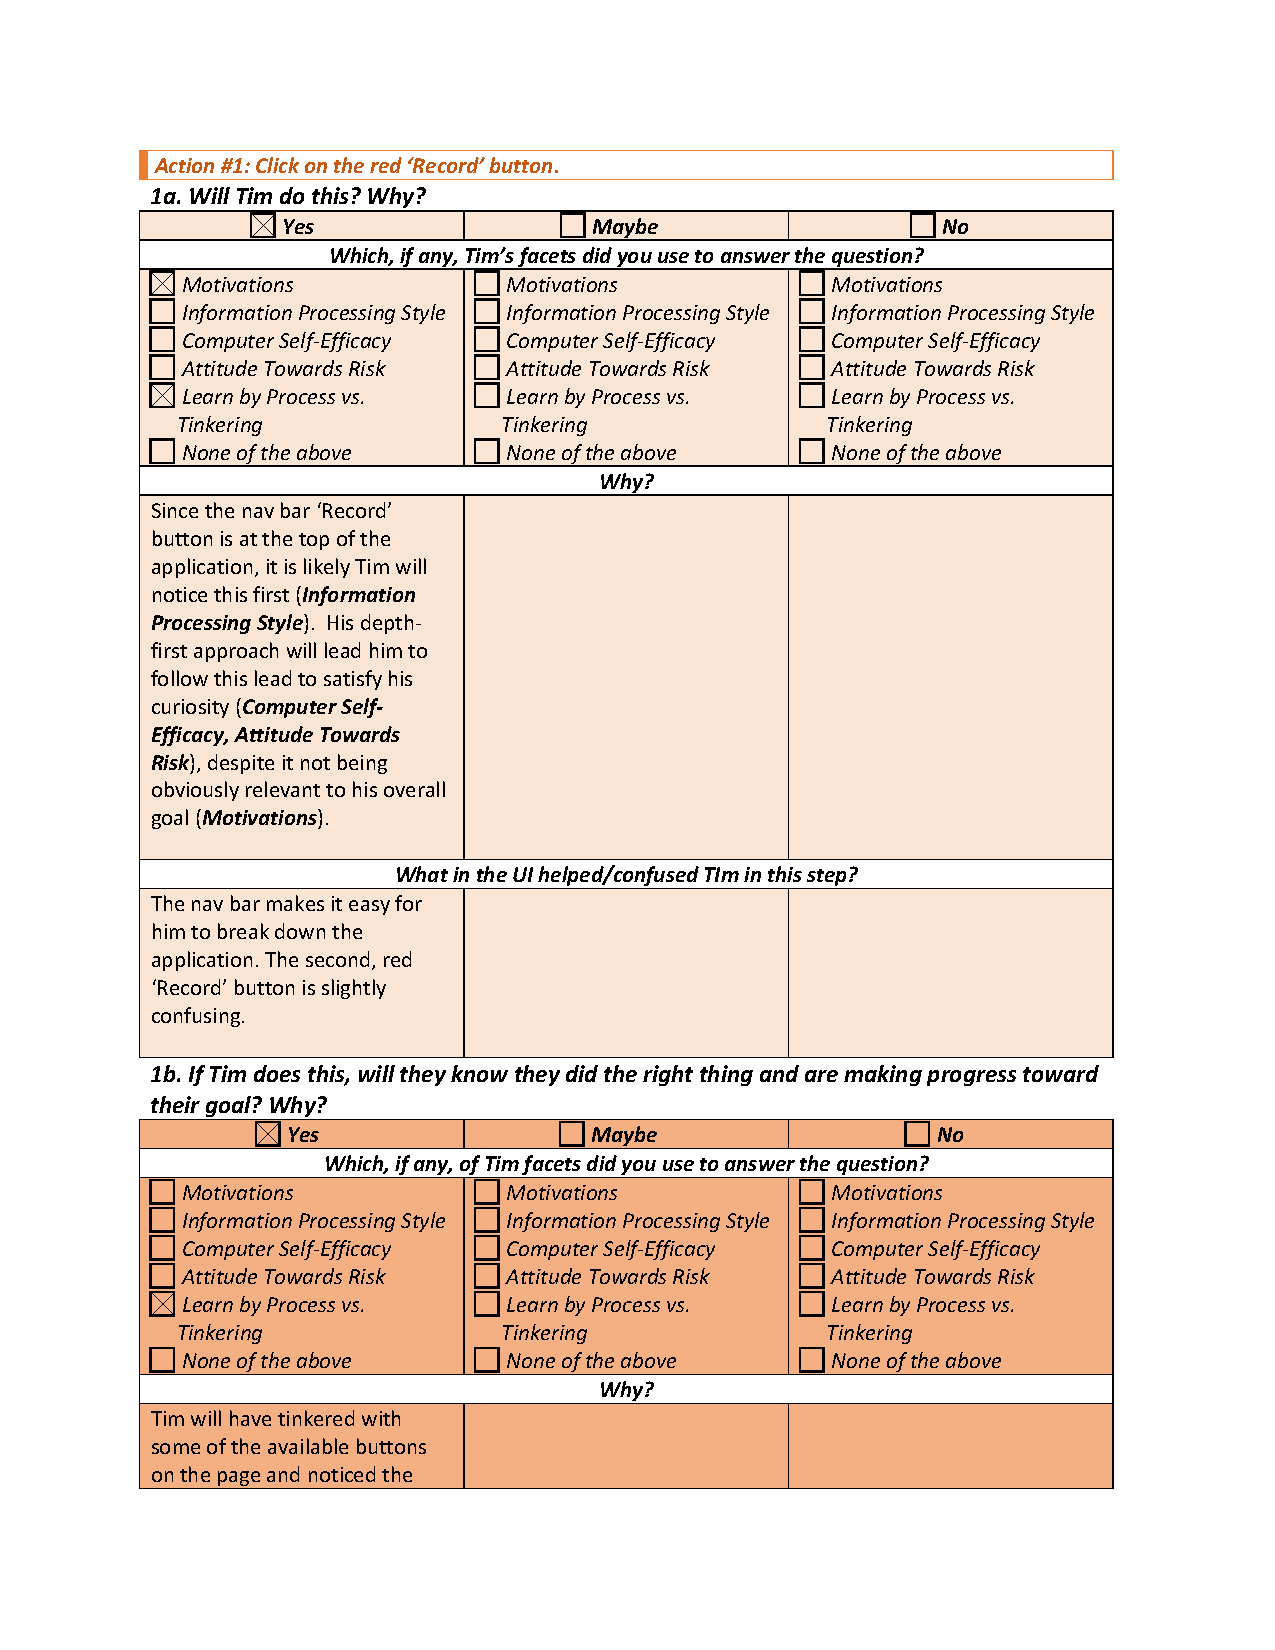
\includepdf[pages=-]{ReportForms/ActionForms/tim-actions.pdf}
\subsubsection{Results Reporting Form}
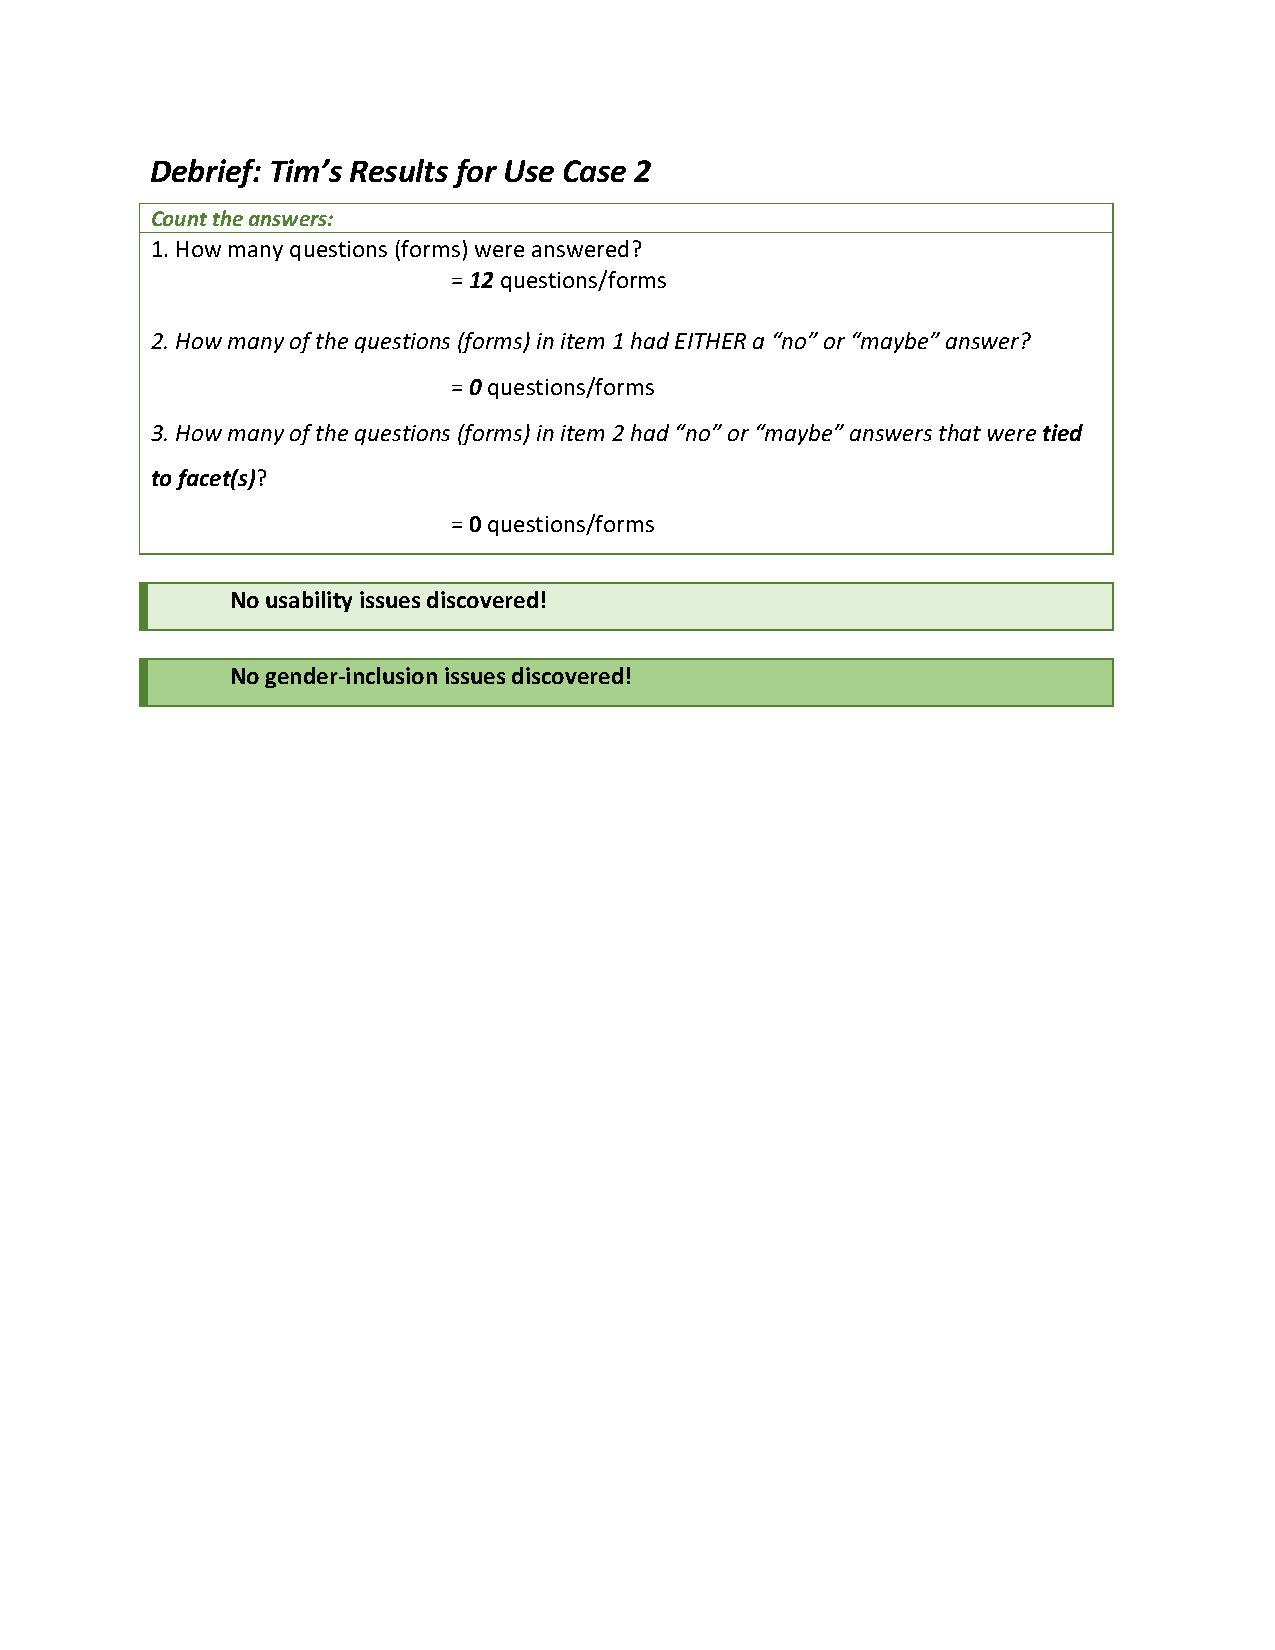
\includepdf[pages=-]{ReportForms/ResultsForms/tim-results.pdf}

\section{Changes Due to GenderMag Evaluation}
Based on the GenderMag evaluation, several issues were identified exclusively for the persona, Abi. This outcome is expected, 
as the Abi persona is specifically designed to target important gender-inclusion challenges through her facets. The evaluation 
revealed four issues, of which the first three relate to gender inclusion, while the fourth is a general usability
matter. The following subsections outline these issues and provides rationale for the associated proposed changes or lack thereof.

\subsection{Subgoal 5: Saving the Recording}
\begin{itemize}
  \item Observation (NO): Abi did not choose to save the recording to a non-default directory.
  \item Rationale: This behavior is observed and although it is related to Abi's facet values and is therefore technically a 
  gender inclusion issue, the team has decided to not consider this a gender inclusion issue as it strictly reflects a personal 
  preference rather than a design barrier.
  \item \textbf{Proposed Change:} No change is proposed, the ability to select a destination remains available to users.
\end{itemize}

\subsection{Action 2b: Visual Feedback on Recording Start}
\begin{itemize}
  \item Observation (MAYBE): After clicking the record button, Abi is unsure whether the recording has started. Although her 
  comprehensive information processing suggests she can infer that a change occurred, the UI does not explicitly confirm that recording 
  has begun.
  \item Rationale: The subtle feedback may negatively impact her self-efficacy. Due to her “learn by process” versus “tinkering” 
  facet, the absence of a clear indicator might cause her to abandon or restart the process.
  \item \textbf{Proposed Change:} Enhance the UI by adding explicit visual feedback (e.g., a clear animation, color change, 
  or status message) immediately after the record button is pressed, to confirm that recording has started.
\end{itemize}

\subsection{Action 3a: Stopping the Recording}
\begin{itemize}
  \item Observation (MAYBE): There is confusion regarding which button stops the recording. While a red button with a 
  stop symbol is present, a previously greyed-out pause button has become interactable and is now colored yellow.
  \item Rationale: This design ambiguity causes uncertainty, particularly for risk-averse users like Abi, 
  who may hesitate or click the wrong button. Clear differentiation between stopping and pausing is essential to 
  avoid wasted effort.
  \item \textbf{Proposed Change:} Redesign the stop function interface by:
  \begin{itemize}
    \item Restoring the pause button to a non-interactable state during recording, or
    \item Differentiating the buttons more clearly using consistent color schemes and intuitive icons so that 
    the stop action is unmistakable.
  \end{itemize}
\end{itemize}

\subsection{Action 5a and 5b: Destination Directory Selection}
\begin{itemize}
  \item Observation (NO): Abi does not engage with the destination directory drop-down menu.
  \item Rationale: This is not a gender inclusion issue but rather a general usability observation. 
  Since the option is available and the decision to select a directory is a matter of personal preference, 
  the design does not restrict user freedom.
  \item \textbf{Proposed Change:} No modifications are proposed.
\end{itemize}

\noindent
\textbf{Summary:} The proposed changes focus on providing clearer feedback during the recording process, 
specifically addressing the start and stop actions, which are directly tied to gender inclusion issues 
identified in the evaluation. The destination directory selection is left unchanged as it does not adversely 
affect user inclusion.

\newpage
\section*{Appendix -- Reflection}
\begin{enumerate}
  \item What lessons did you learn from the GenderMag process that you will carry forward to your Software Engineering career?”
\end{enumerate}

Ian: I learned that methods of testing software usability and accessabilty are constantly evolving and improving. Even if software I
develop in the future might meet some set of current standards, there's is always room for improvement and I have to be aware of, and open to that. \\

Jackson: Through GenderMag, I realized that a one size its all approach in design can (and likely will) overlook critical usability 
issues. Incorporating various user perspectives helps to uncover subtle barriers and improves overall system usability. \\

Mark: Personas are an incredibly valuable tool for usability testing. If real users can't be found or are unavailable, putting youself in the
shoes of different personas is a useful alternative. I'm now aware that even if I develop something solo, I always have the oppourtunity and obligation
to assess the design with different perspectives. \\

Emily: That understanding different user perspectives is essential. The GenderMag process showed the importance of considering 
how different backgrounds and cognitive styles impact software interactions. This awareness will drive me to advocate for inclusive 
design choices in every project. \\
\end{document}